
\documentclass[a4paper,fleqn,usenatbib]{mnras}

\usepackage{newtxtext,newtxmath}
% Depending on your LaTeX fonts installation, you might get better results with one of these:
%\usepackage{mathptmx}
%\usepackage{txfonts}

\usepackage[T1]{fontenc}
\usepackage{ae,aecompl}
\usepackage{booktabs}


\usepackage{graphicx}	% Including figure files
\usepackage{amsmath}	% Advanced maths commands
\usepackage{amssymb}	% Extra maths symbols
\usepackage{color}

%%%%%%%%%%%%%%%%%%%%%%%%%%%%%%%%%%%%%%%%%%%%%%%%%%

%%%%% AUTHORS - PLACE YOUR OWN COMMANDS HERE %%%%%
\usepackage{float}
\newcommand{\todo}[1]{\textcolor{red}{#1}}
\newcommand{\countertodo}[1]{\textcolor{green}{#1}}
\usepackage{adjustbox}
\usepackage{pifont}



\makeatletter
\newcommand{\rmnum}[1]{\romannumeral #1}
\newcommand{\Rmnum}[1]{\expandafter\@slowromancap\romannumeral #1@}
\makeatother

\title[S-process stars in LAMOST]{Discovery of s-process enhanced stars in the LAMOST survey}

\author[Brodie.~J. Norfolk et al.]{Brodie.~J. Norfolk,$^{1}$\thanks{E-mail: bjee7@student.monash.edu (MU)}\thanks{This paper includes data gathered with the 6.5 meter Magellan Telescopes located at Las Campanas Observatory, Chile.}
Andrew.~R. Casey$^{1,2}$,
Matthew ~T. Miles$^{1}$,
Alex ~J. Kemp$^{1}$, \newauthor
Amanda ~I. Karakas$^{1}$,
Kevin ~C. Schlaufman$^{4}$,
Melissa Ness$^{5}$,
Anna Y.~Q. Ho$^{3}$, \newauthor
John ~C. Lattanzio$^{1}$, 
Alexander ~P. Ji$^{6}$
\\
$^{1}$School of Physics \& Astronomy, Monash University, Clayton 3800, Victoria, Australia\\
$^{2}$Faculty of Information Technology, Monash University, Clayton 3800, Victoria, Australia\\
$^{3}$Cahill Center for Astrophysics, California Institute of Technology, MC 249-17, 1200 E California Blvd, Pasadena, Ca, 91125, USA\\
$^{4}$Department of Physics and Astronomy, Johns Hopkins University, 3400 N Charles St., Baltimore, MD 21218, USA
\\
$^{5}$Max-Planck-Institut f\"ur Astronomie, K\"onigstuhl 17, D-69117 Heidelberg, Germany
\\
$^{6}$Carnegie Observatories
}
\date{Accepted XXX. Received YYY; in original form ZZZ}

\pubyear{2018}


\begin{document}
\label{firstpage}
\pagerange{\pageref{firstpage}--\pageref{lastpage}}
\maketitle

\begin{abstract}

In this paper we present the discovery of 967 s-process candidates from 454,180 giant stars observed by LAMOST: this sample constitutes the largest number of s-process enhanced stars ever discovered. We identify these stars in the LAMOST sample by using a data-driven search approach on the spectra directly, and then measure the s-process abundance enhancements using stellar synthesis. Finally, we take advantage of free observing time, and obtain high resolution spectra of a number of candidates. Our sample includes; 257 'barium stars', that are enhanced in both barium and strontium, 49 stars with significant barium enhancement only, and 661 stars which exhibit strontium enhancement only. Our entire barium star stellar sample exists within temperature and luminosity ranges not enveloped by the AGB, which may indicate a recent ($<1\,\textrm{Myr}$) mass accretion event from an AGB companion. Most of our barium stars ($69\%$) show strong carbon enhancements, yet, only 5 candidates ($<2$\,\%) show evidence of sodium enhancement, in contrast with previous claims of preferential sodium enhancement. We argue this may have been a selection bias in previous studies. Our kinematical analysis revealed our stellar sample contains \% disk stars (\% thin and \% thick), and \% halo stars. A comparison with AGB yields suggests the main neutron source responsible for the Ba and Sr enhancements is the $C^{13}(\alpha,n)O^{16}$ reaction chain. Additionally, theoretical models show that this source is dominant in low-mass AGB stars thus, it follows that most of the progenitors of s-process elements in our sample are low-mass AGB stars between $1 - 3\,M_{\odot}$. 

%that the majority of our sample are consistent with Salpeter-like initial mass function, with pollution from a low mass AGB star.

%The abundances of the slow neutron capture process (s-process) elements in stars are a measure of the nucleosynthetic processes that occur primarily in Asymptotic Giant Branch (AGB) stars. Due to their associated enrichment of the s-process element barium, stars with peculiar enhancements of carbon and heavy elements (Z > 30) are historically referred to as 'barium stars'.  Here, we present the discovery of 967 s-process candidates from 454,180 giant stars observed by LAMOST: this sample constitutes the largest number of s-process enhanced stars ever discovered. We identify these stars in the LAMOST sample by using a data-driven search approach on the spectra directly and then measure the s-process abundance enhancements directly using stellar synthesis. Finally, we validate our results using high resolution spectra of a number of candidates. Our sample includes; 257 'barium stars', that are enhanced in both barium and strontium, 49 stars with significant barium enhancement only, and 661 stars which exhibit strontium enhancement only. The unusual chemical abundance patterns of barium stars can be explained if these are in the AGB of stellar evolution. However, many barium stars  have not yet evolved through the red giant phase. Instead, these less evolved 'barium stars' are generally thought to have accreted mass from a more evolved AGB companion.  Our entire barium star stellar sample exists within temperature and luminosity ranges not enveloped by the AGB, which may indicate a recent ($<1\,\textrm{Myr}$) mass accretion event from an AGB companion. These less evolved stars are uniquely informative on the binary fraction, AGB yields, mass transfer and stellar evolution. A comparison with AGB yields suggests that the majority of our sample are consistent with Salpeter-like initial mass function, with pollution from a low mass AGB star. Most of our barium stars (put in percentage) show strong carbon enhancements, consistent with mass transfer from a low-mass AGB companion. Although, only 5 candidates ($<2$\,\%) show evidence of sodium enhancement, in contrast with previous claims of preferential sodium enhancement, we argue this may have been a selection bias in previous studies. When binary properties become available from end-of-mission Gaia astrometry, our sample of s-process stars will be critical in explaining mass transfer in binary systems and refining AGB yields across a range of masses and metallicities.



\end{abstract}

\begin{keywords}
stars: chemically peculiar -- stars: abundances
\end{keywords}

\section{Introduction} \label{sec:intro}

The abundances of the slow neutron capture process (s-process) elements in stars are a measure of the nucleosynthetic processes, that occur primarily in Asymptotic Giant Branch (AGB) stars. Due to their associated enrichment of the s-process element barium, stars with peculiar enhancements of carbon, and heavy elements (Z > 30) are referred to as 'barium stars' as first recognised by \citet{Bidelman1951}. The naming convention associated with barium stars is historical, it is therefore, for the purposes of this paper, necessary to classify definitions used for subsequent discussions. Barium enhanced stars exist as either extrinsic or intrinsic objects, extrinsic barium stars are stellar phenomena exhibiting s-process element enhancement as the result of some polluting process. Stars intrinsically enhanced in barium and other s-process elements are known as AGB S stars. These stars are in the TP-AGB (thermally pulsing-asymptotic giant branch) phase. During this stage of nucleosynthesis, this is an overabundance of both carbon and heavy elements produced through the slow neutron capture process, and exist on the surface as the result of a thermal pulsing cycle. According to the mass-transfer hypothesis, extrinsic barium stars are a consequence of stellar wind accretion \citep{boffin1988,jorissen1992} or Roche-lobe overflow \citep{webbink1986}. Both dynamical systems require a binary configuration a previous TP-AGB companion star (AGB S star), in its final phase as a white dwarf \citep{bohm1980,bohm1984}. In fact, \citet{mcclure1983} determined 85\% of all barium stars exist within binary systems. They further claimed that stellar objects which appeared to be singular are actually pole-on, or highly eccentric binaries with significant radial velocity variations, only occurring in a small ranges as detailed by \citet{pourbaix2004}. For these reasons, the properties and occurrence rate of barium stars are informative of the binary star fraction as a function of metallicity, the mass ratio of binary stars, as well as AGB yields across different masses and metallicities. 

The s-process, occurring in the interior of AGB stars, synthesises roughly half of all elements heavier than iron \citep[e.g.,][]{busso1999,travaglio2001,herwig2005,bisterzo2014,karakas2014}. Late in the AGB phase, during the TP-AGB phase, thermal instabilities occur in the He shell every $10^5$ years or so, depending on the mass of the H-exhausted core. These energy bursts drive a convective zone that sweeps almost the entire region lying between the core and the He-shell, mixing the products of nucleosynthesis within these regions. The energy from the thermal pulses forces the star to expand, pushing the H-shell out to cooler regions and allowing the convective envelope to move inwards to regions previously mixed by the thermal pulse driven convective zones. This phase of expansion and resulting inward movement is defined as the third dredge up (TDU), and is theorised to occur after each thermal pulse. During the TP-AGB phase, surface enrichment in $^{12}$C and heavy elements produced by the s-process, is a result of the repeated inward extensions of TDU \citep[e.g.,][]{busso2001}. The star contracts post dredge up and reignites the H-shell producing the majority of the surface luminosity for the next interpulse period. The interpulse, thermal pulse, and dredge up cycle may occur numerous times, and its frequency is dependent on the initial mass, composition, and mass-loss rate of the star.

Barium giants can form within a metallicity-dependent initial mass range of approximately $0.8 - 8\,M_{\odot}$. The minimum mass for these giants is defined by the mass needed for core helium and carbon burning, which decrease as metallicity decreases. The age of these stars vary considerably, with some as old as $\approx$ 12\,Gyr in metal-poor globular clusters. Metal poor stars enhanced in barium are defined in the literature as CH stars. In contrast, metal-rich, less massive stars may reach ages of $\approx$ 100Myr, this includes stars that are at the core carbon burning limit or very close to it \citep[e.g.,][]{whitelock2013}. Furthermore, metal rich stars enhanced in barium are defined in the literature classically as barium stars.

Many barium stars have been discovered in the disk and halo of the Milky Way \citep{jorissen1993,gomez1997,mennessier1997}. In \citet{pereira2011} it is concluded that metal-rich barium stars share similar kinematics to other metal-rich and super metal-rich stars already analysed, suggesting that they do not belong to the bulge population. It remains necessary to establish known abundances of s-process elements in a greater sample of barium stars in order to: compare their birth rate to theoretical expectations \citep{han1995}, explore the binary fraction at different metallicities, and compare to AGB star yields at different masses and metallicities.
%The relationship between barium stars in the halo \citep[e.g.,][]{junqueira2001,drake2008,pereira2009,allen2006} and metal-poor, yellow, symbiotic halo stars has been established by \citet{jorissen2005} and \citet{pereira2009}.

In this paper we analyse 454,180 giant stars from the second LAMOST data release \citep{luo2015} and identify 967 s-process candidates. In Section \ref{sec:methods}, we describe the observations and candidate selection. Section \ref{sec:observations} details the analysis of high-resolution follow-up observations obtained for a few candidates. In Section \ref{sec:dis}, we discuss the properties of our barium stars in context of existing literature. We provide concluding remarks in Section \ref{sec:con}.

\begin{figure*}
	% To include a figure from a file named example.*
	% Allowable file formats are eps or ps if compiling using latex
	% or pdf, png, jpg if compiling using pdflatex
	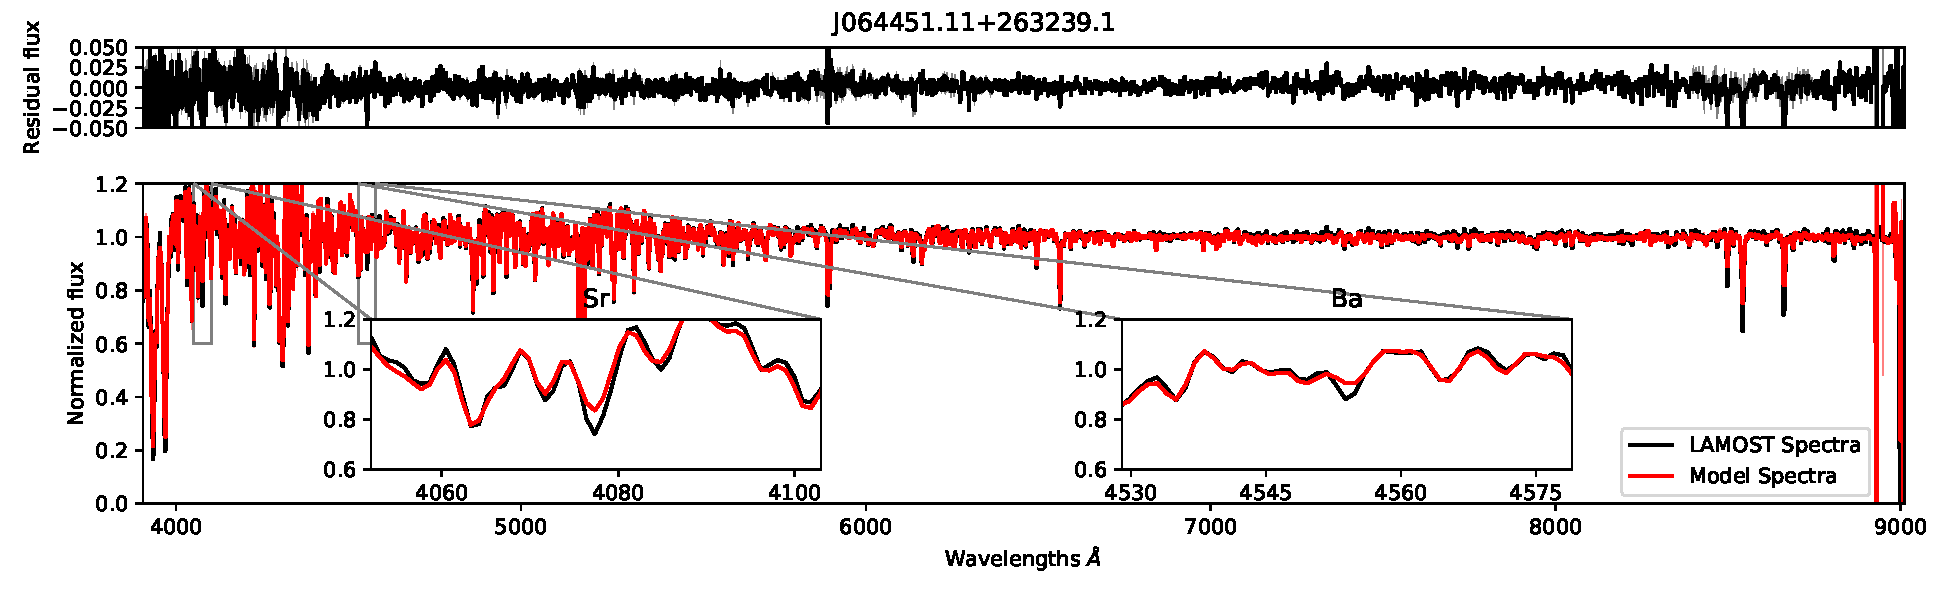
\includegraphics[width=\textwidth]{posterchild_final.pdf}
    \caption{Pseudo-continuum-normalised LAMOST spectra for the s-process candidate J064451.11+263239.2. The data are shown in black and the best-fitting data-driven model is shown in red. We include zoom-in axes to show significant deviations in Sr and Ba at  4077\,\AA\ and 4554\,\AA\, respectively.}
    \label{fig:figure1}
\end{figure*}



\section{Methods} \label{sec:methods}
\subsection{LAMOST analysis}
\subsubsection{Data-driven analysis}
The LAMOST (Large sky Area Multi-Object Fibre Spectrographic) survey released low-resolution ($\mathcal{R} \approx 1800$) optical spectra (3700\,\AA\ to 9000\,\AA) for over two million stars in their second data release \citep{luo2015}. Stellar parameters ($T_{\rm eff}$, $\log{g}$, [M/H], [$\alpha$/M]) were derived using a data-driven model, and constructed using high fidelity APOGEE labels of 9,952 giant stars in common between LAMOST and the APOGEE survey \citep{ho2017}. This data-driven model was used to estimate stellar labels for 454,180 giant stars. We note that this sample is exclusively giant stars, implying that we would not identify dwarf s-process enhanced stars. Cross-validation tests shows that the typical uncertainties are approximately 70\,K in effective temperature $\rm T_{\rm eff}$, 0.1\,dex in surface gravity $\log{g}$, 0.1\,dex in metallicity [M/H], and 0.04\,dex in the $\alpha$-element abundance relative to overall metallicity [$\alpha$/M]. These uncertainties are comparable to the APOGEE uncertainties \citep{alam2015}.


\subsubsection{Candidate selection} \label{sec:cand}
The barium stars analysed in this research were obtained by filtering for significant flux residuals, taken as a disparity between the normalised LAMOST flux and the data driven model, \emph{The Cannon}, derived by \citet{ho2017}. Specifically, we identified barium stars by searching for \ion{Ba}{II} and \ion{Sr}{II} enhancement at the 4554\,\AA\ and 4077\,\AA\ wavelengths, respectively. A negative residual, as shown in a candidate barium star in Figure \ref{fig:figure1}, illustrates an enhancement in the \ion{Ba}{II} and \ion{Sr}{II} lines at 4554\,\AA\, and 4077\,\AA, respectively. These \ion{Ba}{II} and \ion{Sr}{II} resonance lines are very strong, allowing us to identify stars enhanced in neutron-capture elements, given a well-fit model for the data. Stars identified high levels of barium (and not necessarily strontium) required enhancement in both the 4554\,\AA\ and 4934\,\AA\ \ion{Ba}{II} resonance lines, and for stars exclusively enhanced in strontium we looked for significant residuals at the 4077\,\AA\ and 4215\,\AA\ absorption lines.  

We used five filters that each spectrum, for each set of absorption lines, had to meet in order to be considered a s-process rich candidate; these included:


\renewcommand\labelenumi{(\roman{enumi})}
\renewcommand\theenumi\labelenumi

\begin{enumerate} 
\item Profile amplitude for both enhancement lines must be $A < -0.05$.
\item Both amplitudes must be measured within 3$\sigma$ ($|A|/\sigma _A$ < 3).
\item The wavelength at each absorption line must be within 2\,\AA\ ($\lambda$ < 2).
\item The reduced $\chi^2$ from \emph{The Cannon} must be $\chi_r^2 < 3$.
\item And, the LAMOST spectra must have a signal-to-noise ratio of $S/N > 30\,\textrm{pixel}^{-1}$.
\end{enumerate}
In addition, a visual inspection was undertaken to exclude any results containing false positives, candidates exhibiting data reduction issues, apparent absorption finer then the spectral resolution, and overly noisy normalised LAMOST spectra. This combined method generated 967 s-process rich candidates which are provided in Table 1, for which a portion is shown to demonstrate its style and content, it's available online in its entirety. This stellar sample consists of; 257 `barium stars' enhanced in both barium and strontium, 49 stars exhibiting exclusively barium enhancement, and 661 with exclusively strontium enhancement. 

For the remainder of this paper we restrict our analysis to the 257 classical `barium stars' stars that show enhancement in both barium and strontium. While the 49 or 661 stars with only barium or strontium enhancements (respectively) may also be bona fide barium stars, there may be other explanations for their chemical abundance pattern \citep[e.g.,][]{maiorca2011}, and so we restrict our inferences to a `gold sample' of barium stars. 

It's important to note, previous studies \citet{malaney1988} define barium stars through an abundance criteria $\rm[Ba/Fe]\geq +0.3$, and out of our 257 barium star sample using this criteria , only one star ($\rm J092155.95+265253.4$) exhibits a lower [Ba/Fe] of 0.12. However, as previously discussed, a negative residual at the \ion{Ba}{II} resonance line 4554\,\AA\, indicates barium enhancement. Furthermore, as discussed in section \ref{sec:other enhancements}, an enhancement in carbon is observed frequently with barium enhancement. $\rm J092155.95+265253.4$ shows both a negative residual at 4554\,\AA\, and carbon enhancement, we therefore conclude that this single deviant case can be classified as a barium star. Additionally, it should be mentioned, our average abundance error is 0.1, although, these results still indicate our sample can be classified as barium stars since they exhibit enhancement at the BaII resonance line 4554, and have a $\rm[Ba/Fe] \geq 0.2$. Nevertheless, this sample still constitutes the largest collection of barium stars ever discovered, with the next sample of significant size containing 182 barium stars \citep[e.g.,][]{decastro2016}.


\begin{table*}
\centering
\caption{Properties of 967 s-process candidates, the table is available online in its entirety. Here we show a portion to demonstrate its style and content.}
\label{table:table1}
\begin{adjustbox}{width=1\textwidth}
\begin{tabular}{@{}|l|l|c|c|c|c|c|c|c|c|c|c|c|c|c|@{}}
\toprule
2MASSID             & R.~A.         & Dec.        & $v_{r}$ & S/N & $\rm T_{\rm eff}$ & $\log{g}$ & [Fe/H] & [$\alpha$/Fe] & $\chi_r^2$ & [Ba/Fe] & [Sr/Fe] & \ion{Ba}{II} & \ion{Sr}{II} &  \ion{Ba}{II} \& \ion{Sr}{II} \\
& (J2000) & (J2000) & (km\,s$^{-1}$) & (pixel$^{-1}$) & (K)  \\ \midrule
J000019.26+501444.8 & 00:00:19.27 & +50:14:44.9 & -3.9  & 49      & 4973         & 3.27         & 0.21         & 0.08             & 0.66               & 0.25        & 0.83        & \ding{55} & \ding{51}  & \ding{55}   \\
J000020.55+411348.1 & 00:00:20.56 & +41:13:48.2 & -28.2 & 32      & 4882         & 2.74         & -0.22        & 0.04             & 0.23               & -0.17       & 0.90        & \ding{55}& \ding{51}  & \ding{55}    \\
J000134.95+490743.2 & 00:01:34.96 & +49:07:43.2 & -42.3 & 72      & 5044         & 3.11         & -0.54        & 0.11             & 0.79               & 1.02        & 0.45        & \ding{55} & \ding{55} & \ding{51}  \\
J000258.09+410730.0 & 00:02:58.10 & +41:07:30.1 & -34.5 & 41      & 4697         & 2.57         & -0.22        & 0.12             & 0.98               & -0.10       & 0.80        & \ding{55} & \ding{51}  & \ding{55}  \\
J000403.80+160257.1 & 00:04:03.80 & +16:02:57.2 & -35.4 & 42      & 5200         & 3.40         & -0.41        & 0.09             & 0.33               & 0.92        & 0.52        & \ding{55} & \ding{55} & \ding{51}  \\
J000439.16+183350.3 & 00:04:39.17 & +18:33:50.4 & -38.7 & 31      & 4601         & 2.50         & 0.44         & 0.03             & 0.34               & -0.11       & 0.88        & \ding{55} & \ding{51}  & \ding{55}  \\
J000444.87+400402.1 & 00:04:44.88 & +40:04:02.1 & -94.7 & 53      & 4172         & 1.46         & -0.08        & 0.09             & 0.72               & 0.03        & 0.91        & \ding{55} & \ding{51}  & \ding{55}  \\
J000552.76+261849.3 & 00:05:52.76 & +26:18:49.4 & -22.5 & 73      & 4924         & 3.14         & -0.05        & 0.09             & 0.67               & 0.28        & 0.85        & \ding{55} & \ding{51}  & \ding{55}  \\
J000737.70+394055.5 & 00:07:37.70 & +39:40:55.6 & -31.5 & 33      & 4700         & 2.80         & -0.04        & 0.07             & 0.28               & -0.13       & 0.81        & \ding{55} & \ding{51}  & \ding{55}  \\ \hline
\end{tabular}
\end{adjustbox}
\end{table*}

\subsubsection{Enhancements due to sodium, technetium, and carbon} \label{sec:other enhancements}
Enhancements in sodium, technetium, and carbon are useful indicators when determining whether a stellar sample is populated by intrinsically enhanced AGB S stars, or polluted extrinsic barium stars. We performed an identical analysis to the process described in Section \ref{sec:cand} in order to identify sodium, technetium, or carbon enhancement in our sample of 257 barium stars. We used the sodium doublet lines at 5889\,\AA\ and 5895\,\AA\, and required significant absorption in both features. Only 5/257 barium stars met this criteria.

For technetium enhancement we searched for significant residual deviations at 4049\,\AA, 4238\,\AA, 4262\,\AA, 4297\,\AA, and 5924\,\AA. These absorption lines are extremely weak, and would require a substantial amount of technetium enhancement before it would be visible in a high S/N LAMOST spectrum. We found that 51 barium stars exhibited some level of significant enhancement (based on the filters above) at the single technetium line 4238\,\AA, yet none showed enhancement at more than one technetium line. We note that the single enhancement near technetium for these 51 stars may be the consequence of data reduction/calibration artefacts, but we include details of which stars matched on technetium in Table 1 (available online in its entirety) nonetheless.
Finally, for carbon enhancement we searched for significant deviations at the CH and G band near 4300\,\AA. We found 178/257 stars to show significant carbon enhancement (i.e., $[\textrm{C/Fe}] \gtrsim 0.5$). 



\subsubsection{Abundances estimated from LAMOST spectra}
We estimated [Ba/Fe] and [Sr/Fe] abundance ratios for all s-process enhanced candidates by synthesising spectra that would account for the observed flux residuals. We assumed that absorption due to metals is captured by \emph{The Cannon} model, and deviations in flux at the 4554\,\AA\ \ion{Ba}{II} line and the 4077\,\AA\ \ion{Sr}{II} transition are solely due to enhancements in Ba and Sr, respectively \citep{marcs,sme,vald,ispec}. We adopted the stellar parameters ($T_{\rm eff}$, $\log{g}$, [Fe/H]) from \citet{ho2017}, and assume a microturbulence of $v_{mic} = 2\,{\rm km\,s}^{-1}$. Uncertainties in [Ba/Fe] and [Sr/Fe] from LAMOST are taken as the fitting error due to noise, added in quadrature with an adopted $0.2\,{\rm dex}$ systematic error floor.

\subsection{Dynamics}
Using recent astrometry from Gaia/TGAS \citep{gaia2016,gaia2018b, cropper2018, katz2018, lindegren2018, sartoretti2018}, with section filters parallax > 0, and parallax/parallax error >5, we integrated the galactic orbits for 898 s-process enhanced stars. Utilising the \texttt{gala} Python package \citep{price2017}, we integrated each star backwards for $0.5\,\textrm{Gyr}$ in a Milky Way-like potential that consists of four components: a \citet{hernquist1990} bulge and nucleus, a \citet{miyamoto1975} disk, and the \citet{nfw1997} halo. In this potential, the disk and bulge parameters were adjusted to be consistent with previous work \citep{bovy2015}. For our Gaia matched sample, we computed spatial velocities and galactic longitude and latitudes. Spatial velocities are relative to the local standard of rest, where $U_{LSR}$ is positive towards the Galactic centre, $V_{LSR}$ is positive in the direction of Galactic rotation ($l=90^{\circ}, b=0^{\circ}$), and $W_{LSR}$ is positive towards the north galactic pole ($b=90^{\circ}$). Our analysis revealed our stellar sample contains \% disk stars (\% thin and \% thick), and \% halo stars.

\section{Follow-up observations with Magellan/MIKE} \label{sec:observations}

\subsection{Observations and data reduction}
On the night of 07 January 2018 we acquired a high-resolution spectrum of two barium star candidates (J09162834+0259348 and J08351472-0548480) using the MIKE (Magellan Inamori Kyocera Echelle) \citep{bernstein2003} spectrograph on the Magellan Clay telescope \citep{schectman2003} at Las Campanas Observatory, Chile. Candidates for follow-up observations were chosen based on observability constraints and ranked by their apparent visual magnitude, with both candidates having $V \approx 12$. We observed both stars in good seeing using the 0.7 arcsecond slit and 2x2 spatial on-chip binning, providing a spectral resolution of ($\mathcal{R} \approx 28,000$). Exposure times of 100 seconds were sufficient to achieve a S/N ratio exceeding 30 per pixel at 4500\,\AA. We acquired calibration (biases, milky, quartz, and Th-Ar arc lamp) frames in the afternoon. We reduced the data using the \texttt{CarPy} package \citep{kelson2000}. We used spline functions to continuum-normalise all echelle orders, and resampled the normalised spectra onto a uniform-sized wavelength map. We used a rest-frame normalised template of a FGK-type star to place the observed spectra at rest.


\subsection{Abundance analysis}
We adopted the stellar parameters ($T_{\rm eff}$, $\log_{10}g$, [Fe/H]) provided from the data-driven analysis of \citet{ho2017}. Following the procedure outlined in \citet{casey2014}, we measured the strength of \ion{Ba}{II} (4554\,\AA, 4934\,\AA, and 6496\,\AA) and \ion{Sr}{II} (4077\,\AA\ and 4215\,\AA) absorption lines by spectral synthesis, using s-process isotopic ratios from \citet{sneden08}. The abundance ratios we estimate from high-resolution spectra are in excellent agreement with our estimates from LAMOST spectra, all agreeing within the joint $1.2\sigma$. Specifically, for J09162834+02593480 from high- and low-resolution spectra, respectively, we find $[{\rm Sr/Fe}] = 0.76 \pm 0.10$ and $0.85 \pm 0.21$, and $[{\rm Ba/Fe}] = 0.92 \pm 0.10$ and $0.77 \pm 0.21$. The biggest discrepancy we find between high- and low-resolution spectra is [Sr/Fe] for J09162834+0259348, where we find $[{\rm Sr/Fe}] = 0.62 \pm 0.07$ from our Magellan/MIKE spectra, and $0.90 \pm 0.22$ from LAMOST. Finally, for J09162834+0259348 we find $[{\rm Ba/Fe}] = 0.94 \pm 0.12$ from high-resolution spectra and $[{\rm Ba/Fe}] = 0.80 \pm 0.26$ from low-resolution spectra. Uncertainties on abundances derived from high-resolution spectra are taken as the standard deviation of multiple line measurements. The high-resolution abundances we find help validate our methodology for candidate selection, and for estimating abundances from LAMOST spectra.

%\subsubsection{Abundance Uncertainties}


\section{Discussion}  \label{sec:dis}


\subsection{Extrinsic or intrinsic}
Barium enhanced stars exist as either intrinsic or extrinsic stellar objects. Intrinsically enhanced barium stars must be massive enough to reach the TP-AGB phase, and extrinsic barium stars must be in a binary with a previously polluting TP-AGB star companion (AGB S star). Figure \ref{fig:figure2} shows that the majority of our stellar sample exists within temperature and luminosity ranges not enveloped by the AGB. This highlights that our sample does not contain stars to the degree of evolution required to reach the TP-AGB phase, and therefore, must be extrinsic barium stars. However, stars with temperatures below 3800K in Figure \ref{fig:figure2} are potential AGB stars, and their intrinsic or extrinsic nature is not certain. Additionally, it's important to note, previous literature \citep{van2017}, state only 33\% of their stellar sample are post-main-sequence barium stars (extrinsic barium stars). In comparison, we find that all our barium candidates to be extrinsic. This suggests, the construction of our data-driven model may have missed some AGB barium candidates, or that previous studies were biased towards finding luminous AGB S stars. Given that our analysis limits us to only giant stars, such that we do not find any extrinsic barium stars on the main-sequence, na\"ively we would expect that our sample would be biased \emph{towards} finding a higher fraction of red giant stars. Given this bias, Figure \ref{fig:figure3} illustrates through the temperature, and log g ranges present, that our sample is exclusively populated by red giant extrinsic barium stars. This suggests unaccounted selection biases in previous studies towards luminous AGB S stars.

\begin{figure}
	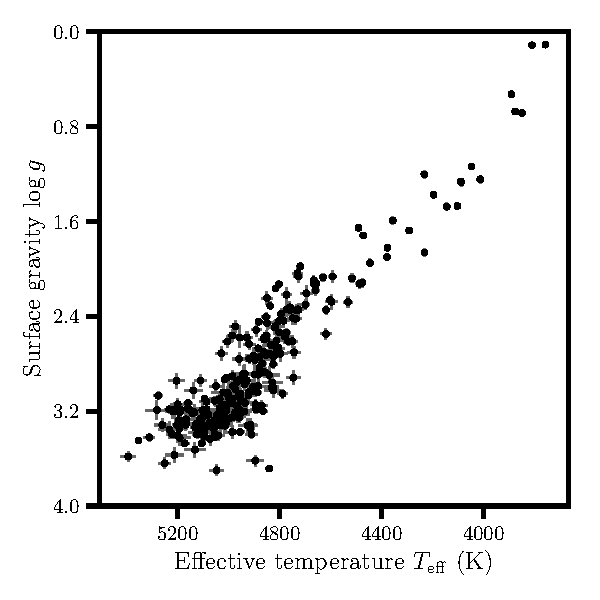
\includegraphics[width=0.5\textwidth]{hrd_new.pdf}
    \caption{Effective temperature $T_{\rm eff}$ and surface gravity $\log{g}$ for 257 candidate barium stars from LAMOST.}
    %Stars with $\log{g} > 2$ (as marked) have not evolved through the thermally pulsing asymptotic giant branch phase, and therefore their abundance signature must be the result of an extrinsic pollution event. The classification of stars with $\log{g} < 2$ would require additional data.}
    \label{fig:figure2}
\end{figure}

\subsection{Sodium enhancement}
Sodium overabundances observed in the atmospheres of giants is thought to be synthesised by the NeNa reaction chain in the convective core of main-sequence stars \citep{el1995}. Sodium is transported to the surface of these giants via mixing during the first dredge-up, and stars with a  minimum mass of $1.5\,M_\odot$ can exhibit enhanced sodium abundances through the NeNa cycle \citep{denissenkov1987,smiljanic2012}. \citet{antipova2004} reported sodium enhancements in 3 of their 16 barium star candidates, and they relate this to the dredge-up of nuclear-burning material produced by convection during the red-giant phase. Moreover, they suggest that [Na/Fe] ratios are systematically higher for giants with lower $\log{g}$ values, however, these [Na/Fe] ratios do not exhibit variations in metallicity. Similarly, \citet{decastro2016} highlights the possible weak anti-correlation between [Na/Fe] ratio and $\log{g}$, and highlights that this trend is present in previous studies \citep[e.g.,][]{boyarchuk2002,mishenina2006,luck2007,takeda2008}.

We find that $<2$\,\% of our barium stars show sodium enhancement, contrary to previous studies \citep[e.g.,][]{decastro2016}, indicating all s-process enhanced stars will exhibit Na enhancement. We also note that the 5 sodium-enhanced barium stars all have values of, $\log{g} \approx 3$, which is inconsistent with the literature. Previous studies suggest, lower $\log{g}$ values are expected, given low $\log{g}$ values systematically contribute to higher [Na/Fe] abundance ratios. It is important to note, sodium enhancement can occur due to the presence of interstellar dust. Using the IRSA's all-sky dust map \citep{schlafly2011}, we find that 2 of 5 of these stars have E(B-V)$\approx$ 0.35, suggesting that the flux residuals around the Na doublet are due to interstellar absorption. However, 3 exhibit low ($\approx$0.045) E(B-V) values, indicating, the enhancement is more likely due to stellar absorption. These results suggest that sodium-rich material from a companion TP-AGB star has polluted these 3 barium candidates, but more importantly, sodium enhancement is by no means ubiquitous in barium stars. However, it should be highlighted that low resolution spectra can result in Na line saturation, limiting the flux enhancement even with an abundance enhancement.

The data that led \citet{decastro2016} to conclude that barium stars have higher [Na/Fe] ratios is subject to systematic differences (biases) between Milky Way studies of normal FGK-type stars, and those focussed on barium stars. This has the potential to contain unresolved differences in the reported [Na/Fe] abundance ratio. These systematic effects would also contribute to the observed correlation between [Na/Fe] and $\log{g}$, since intrinsic barium stars (by definition) have low $\log{g}$ values. We do not observe this correlation between [Na/Fe] and $\log{g}$ in our sample, and we conclude that barium stars do not have higher [Na/Fe] abundance ratios on average.

\subsection{Technetium enhancement}

Technetium has a half life of approximately 211,000 years and as a result, the presence of Tc enhancement is constrained to observations of AGB S stars \citep{jorissen1993} or recently polluted extrinsic barium stars. Our analysis, undertaken for the TC lines 4049\,\AA, 4238\,\AA, 4262\,\AA, 4297\,\AA, and 5924\,\AA, discovered 51 single Tc line matches at 4238,\AA, within our 257 barium star candidate sample. The majority (46/51) have $\log{g} > 2$, suggesting they cannot be AGB S stars, and may indicate a recent ($<1\,\textrm{Myr}$) mass accretion event. However, for Tc to be present in the LAMOST spectra the enhancement must be considerably strong, and given that all 51 matches were at single lines it is concluded that these results are more likely data artefacts. In agreement with previous findings \citep[e.g.,][]{little1987,smith1984,smith1983}, the results indicate that none of the evolved barium stars in our sample exhibited the presence of Tc enhancement, and in accordance with previous literature, it can be concluded that our barium star sample is extrinsic. However, we caution that Tc enhancement is usually a very weak signature, and the presence of Tc would require multiple lines of enhancement. Additionally, it is universally known that numerous Tc lines are considerably blended by other s-process enhancement lines \citep[e.g.,][]{van1999}. 


\begin{figure}
	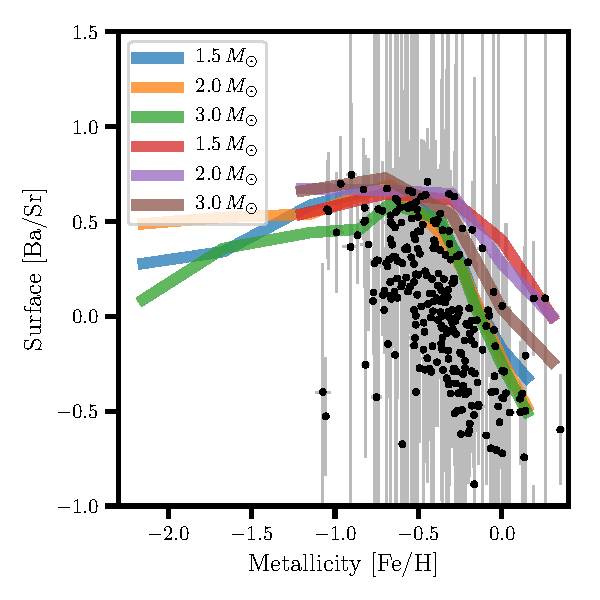
\includegraphics[width=0.5\textwidth]{yields_test.pdf}
    \caption{Metallicities ([Fe/H]; x-axis) and heavy-to-light s-process abundance ratios ([Ba/Sr] as measured from LAMOST; y-axis) for 257 barium star candidates. Coloured lines blue, orange, and green, indicate surface [hs/ls] yields from \citet{cristallo2015} for different masses. Coloured lines red, purple, and brown indicate surface [hs/ls] yields from \citet{karakas_lugaro2016} for [Fe/H] at +0.3. 0.0, and -0.3. From \citet{karakas2018} for [Fe/H] at -0.7, and from \citet{fishlock2014} for [Fe/H] at -1.2.}
    \label{fig:figure3}
\end{figure}

\subsection{Carbon bands}
Barium stars are excellent candidates for investigating the relationship between neutron-capture elements and other species that may be depleted or enhanced, since iron within these stars act as neutron seeds during the operation of the s-process. In the AGB phase the abundance of carbon is a product of helium fusion, specifically the triple-alpha process within a star. In an identical mechanism to the presence of s-process element enhancement, carbon enhanced stars exist intrinsically or extrinsically. Giants and supergiants become enhanced in carbon through TDU process discussed in Section \ref{sec:intro}, and extrinsic carbon enhancement occurs via mass transfer from a binary AGB star. Our analysis produced 178 CH and G band significantly enhanced stars (i.e., $[\textrm{C/Fe}] \gtrsim 0.5$) out of the total 257 barium candidates. These 178 stars exist in a metallicity range of 0 to -1.2, and can be termed "CH stars" in accordance with definitions used in the literature \citep[e.g.][]{luck1991, mcclure1997}.
%Similar to the s-process enhancement, this suggests our candidates are consistent with being either intrinsic or extrinsic Barium stars.


\subsection{Comparison to AGB yields}
AGB stars, and chemically unusual stars that show the chemical signature of mass transfer pollution from a binary AGB companion, highlight the variety of s-process enhancement. In Figure \ref{fig:figure3} we show the heavy-to-light s-process abundance ratio (taken as [Ba/Sr]) for all 257 barium stars identified in LAMOST. Although the [Ba/Sr] ratio is quite noisy, the overall metallicity [Fe/H] is quite precise (0.1\,dex). Despite our LAMOST sample of 454,180 giants having metallicities down to about $[{\rm Fe/H}] = -2$, we only detect barium stars down to metallicities of about $[{\rm Fe/H}] = -1.1$. Given our barium stars exist in this metallicity range of 0 to -1.1, we can classify them as CH stars as defined in previous literature \citep[e.g.][]{luck1991, mcclure1997}.

The final surface s-process index [Ba/Sr], illustrated in Figure \ref{fig:figure3}, illustrates the relationship between [Ba/Sr] yields and the mass of AGB stars. This highlights the main neutron source, the $C^{13}(\alpha,n)O^{16}$ reaction chain, is responsible for the Ba and Sr enhancements. Additionally, theoretical models show that this source is dominant in low-mass AGB stars, and it follows, that most of the progenitors of s-process elements in our sample are low-mass AGB stars between $1 - 3\,M_{\odot}$. However, it's important to note, our results do not indicate when the mass transfer occurred, and our candidates fitting these theoretical yields may not have the correlating binary companion masses. Instead, mass transfer may have occurred early on in the AGB S binary companion star's lifespan, and the resulting [Ba/Sr] abundance present in our barium candidates may reflect pollution from a lower AGB S star mass. Additionally, this can be extended to our candidates not approximated by theoretical yields. Other barium candidates not fitting this relationship represent the possibly more massive, and expectedly rarer, AGB S stars within our sample.

%The Salpeter initial mass function (or any bottom-heavy initial mass function) predicts the majority of stars in the Milky Way will have lower masses, and as predicted the [Ba/Sr] values of our barium stars approximately fit the lower mass yields as seen in Figure \ref{fig:figure3}.

\subsection{Dynamics}

The majority of our sample showed pro-grade orbits that were consistent with membership in the Milky Way disk, indicating they do not originate from an unusual stellar event. Figure \ref{fig:figure4} illustrates the galactic position of each class of s-process enhanced star investigated. For our entire 898 sample, the figure shows \% reside within the galactic disk(\% thin disk and \% thick disk ), and \% within the halo. Our results show similar trends to the literature, samples from \cite{gomez1997} and \cite{mennessier1997} present populations of 75\% contained within the disk, and 25\% within the halo. \cite{pereira2011}’s entire sample resides within the disk, and \cite{decastro2016} states their sample contains 90\% thin disk stars. Although, excluding \cite{decastro2016}’s sample, it is important to note previous studies contain limited stellar populations ranging from 4 to 12 stars, and cannot be representative of the overall galactic position of s-process enhanced stars. \cite{jorissen1993} attributes the galactic position of s-process enhanced stars as dependent on their intrinsic or extrinsic nature, given our sample is entirely extrinsic we cannot comment on the comparison between the two enhancement sources. However, given our extrinsically s-process enhanced sample concentrates towards the galactic plane, we can propose the sample in \cite{jorissen1993} was not large enough to represent the overall galactic position of extrinsic S stars.

\begin{figure}
	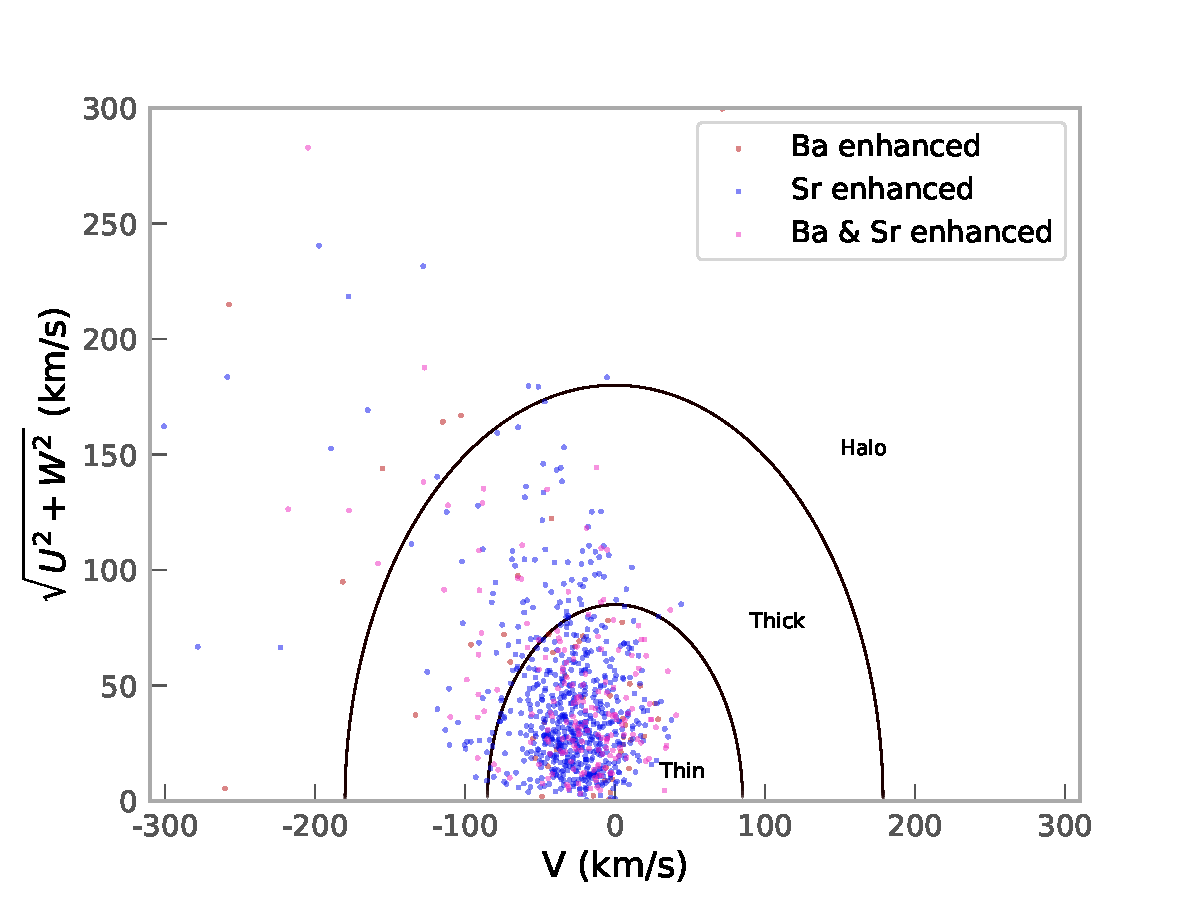
\includegraphics[width=0.5\textwidth]{toomre.pdf}
	\caption{Toomre diagram Spatial velocities ([V (km/s)]; x-axis) and ([$\sqrt{U^2+W^2}$ (km/s)]; y-axis) for number of s-process enhanced candidates matched with Gaia DR2. Coloured markers red, blue, and purple highlight barium, strontium, and both barium and strontium enhancement respectively.}
	\label{fig:figure4}
\end{figure}

\begin{figure}
	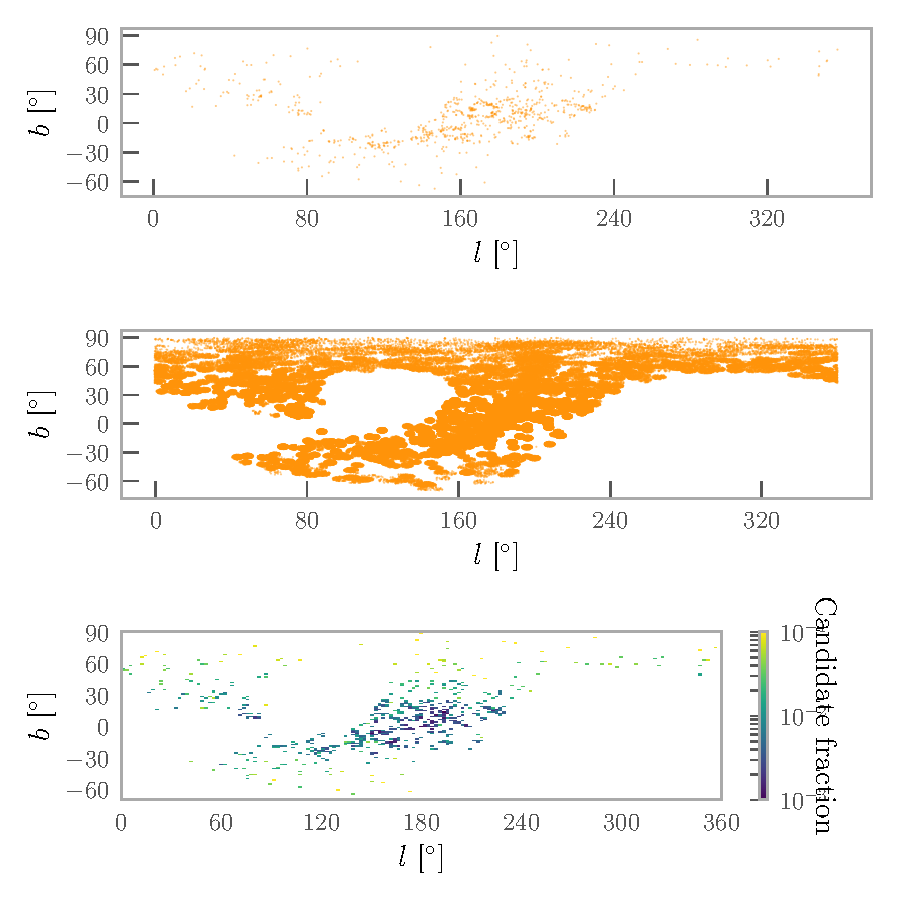
\includegraphics[width=0.5\textwidth]{contour.pdf}
	\caption{Galactic longitude ([$l^{\circ}$]; x-axis) and galactic latitude ([$b^{\circ}$]; y-axis) shown for: number of s-process enhanced candidates matched with Gaia DR2, the LAMOST sample matched with Gaia DR2, and a density contour between the latter two}
	\label{fig:figure5}
\end{figure}

\section{Conclusions} \label{sec:con}

We conducted the largest ever search for s-process enhanced stars using the LAMOST second data release. From 454,180 giant stars, we identify 967 s-process candidates including: 257 stars with significant enhancements in barium and strontium (so-called `barium stars'), 49 stars exhibiting exclusively barium enhancement, and 661 exhibiting exclusively strontium enhancement. This sample size is the greatest total number of barium stars known, and represents the largest sample of s-process enhanced stars to date.  Our kinematical analysis revealed our stellar sample contains \% disk stars (\% thin and \% thick), and \% halo stars, indicating our barium stars were not produced through an unusual galactic event. 

We find 178/257 barium star candidates show carbon enhancement, consistent with the literature, and are possible CH stars. However, in contrast with previous works, we do not find barium stars to have significantly higher [Na/Fe] than Milky Way field giants. Only 5/257 of our barium stars show enhancement in Na, and the flux residuals in three of those are likely due to interstellar dust. We suggest that biases between literature sources and systematic effects in measuring [Na/Fe] from stars with low $\log{g}$ contributed to this effect. 

Despite our noisy estimates of [Ba/Fe] and [Sr/Fe] from LAMOST spectra, comparisons with AGB yields indicate the main neutron source responsible for the Ba and Sr enhancements, the $C^{13}(\alpha,n)O^{16}$ reaction chain, and theoretical yields suggest the progenitors of our s-process enhanced sample are low-mass AGB stars, between $1 - 3\,M_{\odot}$. We encourage follow-up observations with high-resolution spectrographs in order to precisely measure a full suite of neutron-capture abundances. This data would permit the most detailed comparisons with AGB star yields ever considered.

 

\section*{Acknowledgements}
We thank David W. Hogg (NYU) and Hans-Walter Rix (MPIA) for useful discussions. 
A.~R.~C. is supported through an Australian Research Council Discovery Project under grant DP160100637.
A. Y. Q. H. was supported by the GROWTH project funded by the National Science Foundation under PIRE Grant No 1545949, and a National Science Foundation Graduate Research Fellowship under Grant No. DGE-1144469. 
This research has made use of NASA's Astrophysics Data System.
Guoshoujing Telescope (the Large Sky Area Multi-Object Fiber Spectroscopic Telescope LAMOST) is a National Major Scientific Project built by the Chinese Academy of Sciences. Funding for the project has been provided by the National Development and Reform Commission. LAMOST is operated and managed by the National Astronomical Observatories, Chinese Academy of Sciences. 
This work has made use of data from the European Space Agency (ESA) mission
{\it Gaia} (\url{https://www.cosmos.esa.int/gaia}), processed by the {\it Gaia}
Data Processing and Analysis Consortium (DPAC,
\url{https://www.cosmos.esa.int/web/gaia/dpac/consortium}). Funding for the DPAC
has been provided by national institutions, in particular the institutions
participating in the {\it Gaia} Multilateral Agreement.


 
\bibliographystyle{mnras}
%\bibliography{example} % if your bibtex file is called example.bib

\begin{thebibliography}{99}
\bibitem[Alam et al.(2015)]{alam2015} Alam, S., Albareti, F.~D., Allende Prieto, C., et al.\ 2015, \apjs, 219, 12 
%\bibitem[\protect\citeauthoryear{Allen \& Barbuy}{2006}]{allen2006}
%Allen, D.~M.,\& Barbuy B. 2006, 
%A$\&$A, 454, 917
\bibitem[\protect\citeauthoryear{Antipova et al.}{2004}]{antipova2004}
Antipova, L.~I., Boyarchuk, A.~A., Pakhomov, Yu.~V.,\& Panchuk, V.~E. 2004, 
ARep, 48, 597
\bibitem[\protect\citeauthoryear{Bernstein et al.}{2003}]{bernstein2003}
Bernstein, R., Shectman, S.~A., Gunnels, S.~M., Mochnacki, S.,\& Athey, A.~E. 2003, 
SPIE, 4841, 1694    
\bibitem[\protect\citeauthoryear{Bidelman \& Keenan}{1951}]{Bidelman1951}
Bidelman, W.~P. \& Keenan, P.~C. , 1951, ApJ, 114, 473
\bibitem[\protect\citeauthoryear{Bisterzo et al.}{2014}]{bisterzo2014}
Bisterzo, S., et al. 2014, 
ApJ, 787, 10
A$\&$A, 424, 727
\bibitem[Blanco-Cuaresma et al.(2014)]{ispec} Blanco-Cuaresma, S., Soubiran, C., Heiter, U., \& Jofr{\'e}, P.\ 2014, \aap, 569, A111 
\bibitem[\protect\citeauthoryear{Boffin \& Jorissen}{1988}]{boffin1988}
Boffin H, M.~J.,\& Jorissen, A. 1988, 
A$\&$A, 205, 155
\bibitem[\protect\citeauthoryear{B\"ohm-Vitense}{1980}]{bohm1980}
B\"ohm-Vitense, E. 1980, 
ApJ, 239, L79
\bibitem[\protect\citeauthoryear{B\"ohm-Vitense et al.}{1984}]{bohm1984}
B\"ohm-Vitense, E., Nemec, J.,\& Proffitt, C. 1984, 
ApJ, 278, 726
\bibitem[\protect\citeauthoryear{Bovy}{2015}]{bovy2015}
Bovy, J. 2015, 
ApJ, 216, 29
\bibitem[\protect\citeauthoryear{Boyarchuk et al.}{2002}]{boyarchuk2002}
Boyarchuk, A.~A., Pakhomov, Y.~V., Antipova, L.~I.,\& Boyarchuk, M.~E. 2002, 
ARep, 46, 819
\bibitem[\protect\citeauthoryear{Busso et al.}{1999}]{busso1999}
Busso, M., Gallino, R., \& Wasserburg, P.~C. 1999, 
ARA$\&$A, 37, 239
\bibitem[\protect\citeauthoryear{Busso et al.}{2001}]{busso2001}
Busso, M., Gallino, R., Lambert, D.~L., Travaglio, C.\& Smith, V.~V. 2001, 
ApJ, 557, 802
\bibitem[\protect\citeauthoryear{Casey}{2014}]{casey2014}
Casey, A.~R. 2014, 
PhD Thesis, Australian National University
\bibitem[\protect\citeauthoryear{Cristallo et al.}{2015}]{cristallo2015}
Cristallo, S., Straniero, O., Piersanti, L.,\& Gobrecht, D. 2015, 
ApJ, 219, 40
\bibitem[\protect\citeauthoryear{Cropper et al.}{2018}]{cropper2018}
Cropper, M., Katz, D., Sartoretti, P., Prusti, T., de Bruijne, J.~H.~J., Chassat, F., Charvet, P., Boyadijan, J., Perryman, M., Sarri, G., Gare, P., Erdmann, M., Munari, U., Zwitter, T., Wilkinson, M., Arenou, F., Vallenari, A., G{\'o}mez, A., Panuzzo, P., Seabroke, G., Allende Prieto, C., Benson, K., Marchal, O., Huckle, H., Smith, M., Dolding, C., Jan{\ss}en, K., Viala, Y., Blomme, R., Baker, S., Boudreault, S., Crifo, F., Soubiran, C., Fr{\'e}mat, Y., Jasniewicz, G., Guerrier, A., Guy, L.~P., Turon, C., Jean-Antoine-Piccolo, A., Th{\'e}venin, F., David, M. Gosset, E.,\& Damerdji, Y. 2018
\bibitem[\protect\citeauthoryear{deCastro et al.}{2016}]{decastro2016}
deCastro, D.~B., Pereira, C.~B., Roig, F., Jilinski, E., Drake, N.~A., Chavero, C.,\& Sales Silva, J.~V. 2016, 
MNRAS, 459, 4299
\bibitem[\protect\citeauthoryear{Denissenkov \& Ivanov}{1987}]{denissenkov1987}
Denissenkov P.~A.,\& Ivanov, V.~V. 1987, 
SvAL, 13, 214
%\bibitem[\protect\citeauthoryear{Drake \& Pereira}{2008}]{drake2008}
%Drake N.,~A.,\& Pereira, C.~B. 2008, 
%AJ, 135, 1070
\bibitem[\protect\citeauthoryear{El Eid \& Champagne}{1995}]{el1995}
El Eid, M.~F.,\& Champagne, A.~E. 1995, 
ApJ, 451, 298
\bibitem[\protect\citeauthoryear{Fishlock et al}{2014}]{fishlock2014}
Fishlock, C.~K., Karakas, A.~I., Lugaro, M.,\& Yong, D. 2014, 
ApJ, 797, 44
\bibitem[\protect\citeauthoryear{Gaia Collaboration et al.}{2016}]{gaia2016}
Gaia Collaboration, Prusti, T., de Bruijne, J.~H.~J., Brown, A.~G.~A., Vallenari, A., Babusiaux, C., Bailer-Jones, C.~A.~L., Bastian, U., Biermann, M.,\& Evans, D.~W. et al. 2016, 
A$\&$A, 595, A1
\bibitem[\protect\citeauthoryear{Gaia Collaboration et al.}{2018b}]{gaia2018b}
Gaia Collaboration, Brown, A.~G.~A., Vallenari, A, Prusti, T., de Bruijne, J.~H.~J., Babusiaux, C.,\& Bailer-Jones, C.~A.~L. 2018, 
\bibitem[Gustafsson et al.(2008)]{marcs} Gustafsson, B., Edvardsson, B., Eriksson, K., et al.\ 2008, \aap, 486, 951 
\bibitem[\protect\citeauthoryear{Gomez et al.}{1997}]{gomez1997}
Gomez, A.~E., Luri, X., Grenier, S., et al. 1997, 
A$\&$A, 319, 881
\bibitem[\protect\citeauthoryear{Han et al.}{1995}]{han1995}
Han, Z., Eggleton, P.~P., Podsiadlowski, P.,\& Tout, C.~A. 1995, 
MNRAS, 277, 1443
\bibitem[\protect\citeauthoryear{Hernquist}{1990}]{hernquist1990}
Hernquist, L. 1990, 
ApJ, 356, 359
\bibitem[\protect\citeauthoryear{Herwig}{2005}]{herwig2005}
Herwig, F. 2005, 
ARA$\&$A, 43, 435
\bibitem[\protect\citeauthoryear{Ho et al.}{2017}]{ho2017}
Ho, A.~Y.~Q., Ness, M.~K., Hogg, D.~W., Rix, H.-W. Liu, C., Yang, F., Zhang, Y., Hou, Y.,\& Wang, Y. 2017, 
ApJ, 836, 5
\bibitem[\protect\citeauthoryear{Jorissen \& Boffin}{1992}]{jorissen1992}
Jorissen, A.,\& Boffin H, M.~J., 1992, 
Evidences for interaction among wide binary systems: To Ba or not to Ba? In: Duquennoy, A., Mayor, M.,(eds.) Binaries as tracers of stellar formation. Cambridge Univ. Press., p.185
\bibitem[\protect\citeauthoryear{Jorissen et al.}{1993}]{jorissen1993}
Jorissen, A., Frayer, D.~T., Johnson, H.~W., Mayor, M.,\& Smith, V.~V. 1993, 
A$\&$A, 271, 463
\bibitem[\protect\citeauthoryear{Jorissen et al.}{2005}]{jorissen2005}
Jorissen, A., Za$\check{c}$, L., Udry, S., Lindgren, H.,\& Musaev, F.~A. 2005, 
A$\&$A, 441, 1135
%\bibitem[\protect\citeauthoryear{Junqueira \& Pereira}{2001}]{junqueira2001}
%Junqueira S.,\& Pereira, C.~B. 2001, 
%AJ, 122, 360
\bibitem[\protect\citeauthoryear{Karakas \& Lattanzio}{2014}]{karakas2014}
Karakas, A.~I.,\& Lattanzio C.~J. 2014, 
PASA, 31, 30
\bibitem[\protect\citeauthoryear{Karakas \& Lugaro}{2016}]{karakas_lugaro2016}
Karakas, A.~I.,\& Lugaro M. 2016, 
ApJS, 825, 26
\bibitem[\protect\citeauthoryear{Karakas et al.}{2018}]{karakas2018}
Karakas, A.~I. 2018, 
MNRAS, submitted
\bibitem[\protect\citeauthoryear{Katz et al.}{2018}]{katz2018}
Katz, D., Sartoretti, P., Cropper, M., Panuzzo, P., Seabroke, G.~M., Viala, Y., Benson, K., Blomme, R., Jasniewicz, G., Jean-Antoine, A., Huckle, H., Smith, M., Baker, S., Crifo, F., Damerdji, Y., David, M., Dolding, C., Fr{\'e}mat, Y., Gosset, E., Guerrier, A., Guy, L.~P., Haigron, R., Jan{\ss}en, K., Marchal, O., Plum, G., Soubiran, C., Th{\'e}venin, F. ,Ajaj, M., Allende Prieto, C., Babusiaux, C., Boudreault, S., Chemin, L., Delle Luche, C., Fabre, C., Gueguen, A., Hambly, N.~C., Lasne, Y., Meynadier, F., Pailler, F., Panem, C., Royer, F., Tauran, G., Zurbach, C., Zwitter, T., Arenou, F., Bossini, D., Gomez, A., Lemaitre, V., Leclerc, N., Morel, T., Munari, U., Turon, C., Vallenari, A.,\& {\v Z}erjal, M. 2018
\bibitem[\protect\citeauthoryear{Kelson et al.}{2000}]{kelson2000}
Kelson, D.~D., Illingworth, G.~D., van Dokkum, P.~G.,\& Franx, M. 2000, ApJ, 531, 159
%\bibitem[\protect\citeauthoryear{Kelson}{2003}]{kelson2003}
%Kelson, D.~D. 2003, 
%PASP, 115, 688
%\bibitem[\protect\citeauthoryear{Kobayashi et al.}{2011}]{kobayashi2011}
%Kobayashi, C., Karakas, A., \& Umeda, H. 2011, 
%MNRAS, 414, 3231
\bibitem[Kupka et al.(1999)]{vald} Kupka, F., Piskunov, N., Ryabchikova, T.~A., Stempels, H.~C., \& Weiss, W.~W.\ 1999, \aaps, 138, 119 
\bibitem[\protect\citeauthoryear{Lindegren et al.}{2018}]{lindegren2018}
Lindegren, L., Hernandez, J., Bombrun, A., Klioner, S., Bastian, U., Ramos-Lerate, M., de Torres, A., Steidelmuller, H, Stephenson, C., Hobbs, D., Lammers, U., Biermann, M. ,Geyer, R., Hilger, T., Michalik, D., Stampa, U., McMillan, P.~J., Castaneda, J., Clotet, M., Comoretto, G., Davidson, M., Fabricius, C., Gracia, G., Hambly, N.~C., Hutton, A., Mora, A., Portell, J., van Leeuwen, F., Abbas, U., Abreu, A., Altmann, M., Andrei, A., Anglada, E., Balaguer-Nunez, L., Barache, C., Becciani, U., Bertone, S., Bianchi, L., Bouquillon, S., Bourda, G., Brusemeister, T., Bucciarelli, B., Busonero, D., Buzzi, R., Cancelliere, R., Carlucci, T., Charlot, P., Cheek, N., Crosta, M., Crowley, C., de Bruijne, J., de Felice, F., Drimmel, R. Esquej, P., Fienga, A., Fraile, E., Gai, M., Garralda, N., Gonzalez-Vidal, J.~J., Guerra, R., Hauser, M., Hofmann, W., Holl, B., Jordan, S., Lattanzi, M.~G., Lenhardt, H., Liao, S., Licata, E., Lister, T., Loffler, W., Marchant, J., Martin-Fleitas, J.-M., Messineo, R., Mignard, F., Morbidelli, R., Poggio, E., Riva, A., Rowell, N., Salguero, E., Sarasso, M., Sciacca, E., Siddiqui, H., Smart, R.~L., Spagna, A., Steele, I., Taris, F., Torra, J., van Elteren, A., van Reeven, W.,\& Vecchiato, A. 2018
\bibitem[\protect\citeauthoryear{Little-Marenin \& Little}{1987}]{little1987}
Little-Marenin, I.~R.,\& Little, S.~J. 1987, 
AJ, 93, 1539
\bibitem[\protect\citeauthoryear{Luck \& Bond}{1991}]{luck1991}
Luck R.~E.,\& Bond, H.~E. 1991, 
ApJS, 77, 515
\bibitem[\protect\citeauthoryear{Luck \& Heiter}{2007}]{luck2007}
Luck R.~E.,\& Heiter, U. 2007, 
AJ, 133, 2464
\bibitem[\protect\citeauthoryear{Luo et al}{2015}]{luo2015}
Luo, A.~L., Bai, Z.~R., et al. 2015, 
RAA, in press
\bibitem[Maiorca et al.(2011)]{maiorca2011} Maiorca, E., Randich, S., Busso, M., Magrini, L., \& Palmerini, S.\ 2011, \apj, 736, 120 
\bibitem[\protect\citeauthoryear{Malaney \& Lambert}{1988}]{malaney1988}
Malaney, R.~A.,\& Lambert, D.~L. 1988, 
MNRAS, 235, 695
\bibitem[\protect\citeauthoryear{McClure}{1983}]{mcclure1983}
McClure, R.~D. 1983, 
ApJ, 268, 264
\bibitem[\protect\citeauthoryear{McClure}{1997}]{mcclure1997}
McClure, R.~D. 1997, 
PASP, 109, 536
\bibitem[\protect\citeauthoryear{Mennessier et al.}{1997}]{mennessier1997}
Mennessier, M.~O., Luri, X., Figueras, F., et al. 1997, 
A$\&$A, 326, 722
\bibitem[\protect\citeauthoryear{Mishenina et al.}{2006}]{mishenina2006}
Mishenina, T.~V., Bienaym\' e, O., Gorbaneva, T.~I.,\& Charbonnel, C. 2006, 
A$\&$A, 456, 1109
\bibitem[\protect\citeauthoryear{Miyamoto-Nagai}{1975}]{miyamoto1975}
Miyamoto, M,\& Nagai, R. 1975, 
PASJ, 27, 533
\bibitem[\protect\citeauthoryear{Navarro, Frenk \& White}{1997}]{nfw1997}
Navarro, J.~F., Frenk, C.~S.,\& White, S.~D.~M. 1997, 
ApJ, 490, 493
%\bibitem[\protect\citeauthoryear{Pereira \& Drake}{2009}]{pereira2009}
%Pereira, C.~B.,\& Drake N.,~A. 2009, 
%A$\&$A, 496, 791
\bibitem[\protect\citeauthoryear{Pereira et al.}{2011}]{pereira2011}
Pereira, C.~B., Sales Silva, J.,~A., Chavero, C., Roig, F.,\& Jilinski E. 2011, 
A$\&$A, 533, A51
\bibitem[\protect\citeauthoryear{Pourbaix et al.}{2004}]{pourbaix2004}
Pourbaix, D., Tokovinin, A.~A., Batten, A.~H., Fekel, F.~C., Hartkopf, W.~I. et al. 2001, 
%\bibitem[\protect\citeauthoryear{Prantzos}{2012}]{prantzos2012}
%Prantzos, N. 2012, 
%A$\&$A, 542, A67
\bibitem[\protect\citeauthoryear{Price-Whelan}{2017}]{price2017}
Price-Whelan, A.~M. 2017, 
The Journal of Open Source Software, 2, 388
%\bibitem[\protect\citeauthoryear{Romano et al.}{2010}]{romano2010}
%Romano, D., et al. 2010, 
%A$\&$A, 522, A32
\bibitem[\protect\citeauthoryear{Sartoretti et al.}{2018}]{sartoretti2018}
Sartoretti, P., Katz, D., Cropper, M., Panuzzo, P., Seabroke, G.~M. ,Viala, Y., Benson, K., Blomme, R., Jasniewicz, G., Jean-Antoine, A., Huckle, H., Smith, M., Baker, S., Crifo, F., Damerdji, Y., David, M., Dolding, C., Fremat, Y., Gosset, E., Guerrier, A., Guy, L.~P., Haigron, R., Janssen, K., Marchal, O., Plum, G., Soubiran, C., Thevenin, F., Ajaj, M., Allende Prieto, C., Babusiaux, C., Boudreault, S., Chemin, L., Delle Luche, C., Fabre, C., Gueguen, A., Hambly, N.~C., Lasne, Y., Meynadier, F., Pailler, F., Panem, C., Riclet, F., Royer, F., Tauran, G., Zurbach, C., Zwitter, T., Arenou, F., Gomez, A., Lemaitre, V., Leclerc, N., Morel, T., Munari, U., Turon, C.,\& Zerjal, M. 2018
\bibitem[\protect\citeauthoryear{Schectman \& Johns}{2003}]{schectman2003}
Shectman, S.~A.,\& Johns, M. 2003, 
SPIE, 4837, 910
\bibitem[\protect\citeauthoryear{Schlafly \& Finkbeiner}{2011}]{schlafly2011}
Schlafly, E.~F.,\& Finkbeiner, D.~P. 2011, 
Apj, 737, 103
\bibitem[\protect\citeauthoryear{Smiljanic}{2012}]{smiljanic2012}
Smiljanic, R. 2012, 
MNRAS, 422, 1562
\bibitem[\protect\citeauthoryear{Smith \& Wallerstein}{1983}]{smith1983}
Smith, V.~V.,\& Wallerstein, G. 1983, 
ApJ, 273, 742
\bibitem[\protect\citeauthoryear{Smith}{1984}]{smith1984}
Smith, V.~V. 1984, 
A$\&$A, 132, 326
\bibitem[Sneden et al.(2008)]{sneden08} Sneden, C., Cowan, J.~J., \& Gallino, R.\ 2008, \araa, 46, 241 
\bibitem[\protect\citeauthoryear{Takeda et al.}{2008}]{takeda2008}
Takeda, Y., Sato, B.~V.,\& Murata, D. 2008, 
AJ, 60, 781
\bibitem[\protect\citeauthoryear{Travaglio et al.}{2001}]{travaglio2001}
Travaglio, C., et al. 2001, 
ApJ, 549, 346
\bibitem[\protect\citeauthoryear{Webbink}{1986}]{webbink1986}
Webbink, R.~F. 1986, 
In: Leung, K.~C., Zhai, D.~S.(eds.) Critical Observations versus Physical Models for Close Binary Systems. Gordon and Breach, New York, p.403
\bibitem[\protect\citeauthoryear{Whitelock et al.}{2013}]{whitelock2013}
Whitelock, P.~A., et al. 2013, 
MNRAS, 428, 2216
\bibitem[Valenti \& Piskunov(1996)]{sme} Valenti, J.~A., \& Piskunov, N.\ 1996, \aaps, 118, 595 
\bibitem[\protect\citeauthoryear{Van Eck \& Jorissen}{1999}]{van1999}
Van Eck, S. \& Jorissen, A. 1999, 
A$\&$A, 345, 127
\bibitem[\protect\citeauthoryear{Van der Swaelmen et al.}{2017}]{van2017}
Van der Swaelmen, M., Boffin, H.~M.~J., Jorissen, A.,\& Van Eck, S. 2017, 
A$\&$A, 597, A68
\end{thebibliography}
% Don't change these lines
\bsp	% typesetting comment
\label{lastpage}
\end{document}